\documentclass{article}
\usepackage[utf8]{inputenc}
\usepackage{geometry}
\usepackage{hyperref}
\usepackage{multicol}
\usepackage{graphicx}
\usepackage{float}

\geometry{a4paper, total={170mm,257mm}, left=20mm, top=20mm}
\usepackage{graphicx}
\usepackage{titling}

\title{Group A3D: SPARQL Queries and Analytics}
\author{Group A3D}
\date{10th January 2025}

 \usepackage{fancyhdr}
\fancypagestyle{plain}{%  the preset of fancyhdr
    \fancyhf{} % clear all header and footer fields
    % \fancyfoot[R]{\includegraphics[width=2cm]{KULEUVEN_GENT_RGB_LOGO.png}}
    \fancyhead[]{\thedate}
    \fancyhead[L]{SPARQL Queries and Analytics}
    \fancyhead[R]{\theauthor}
}
\makeatletter
\def\@maketitle{%
  \newpage
  \null
  \vskip 1em%
  \begin{center}%
  \let \footnote \thanks
    {\LARGE \@title \par}%
    \vskip 1em%
    %{\large \@date}%
  \end{center}%
  \par
  \vskip 1em}
\makeatother

\usepackage{lipsum}
\usepackage{cmbright}

\usepackage{xcolor}
\usepackage{listings}
\lstdefinelanguage{SPARQL}{
    keywords={SELECT, WHERE, AS, FILTER, OPTIONAL, GRAPH, UNION, PREFIX, ORDER, BY, ASC, DESC, LIMIT, OFFSET, BIND, GROUP, HAVING, COUNT, DISTINCT, SUM, AVG, MIN, MAX, GROUP_CONCAT, SEPARATOR},
    keywordstyle=\color{blue}\bfseries,
    ndkeywords={a, rdf:type},
    ndkeywordstyle=\color{teal}\bfseries,
    identifierstyle=\color{black},
    stringstyle=\color{red}\ttfamily,
    commentstyle=\color{gray}\itshape,
    sensitive=true,
    morecomment=[l][\color{gray}]
}
\lstset{
    language=SPARQL,
    basicstyle=\ttfamily\small,
    numbers=left,
    numberstyle=\tiny\color{gray},
    stepnumber=1,
    frame=single,
    breaklines=true,
    captionpos=b,
    tabsize=2,
    showstringspaces=false
}

\begin{document}

\maketitle

\begin{tabular}{@{}ll}
	\textbf{Group members:}
	 & \href{mailto:andrea.bruttomesso.1@studenti.unipd.it}{Andrea Bruttomesso} 2120933 \\
	 & \href{mailto:alessandro.corro.1@studenti.unipd.it}{Alessandro Corr\`o} 2125034   \\
	 & \href{mailto:davide.seghetto@studenti.unipd.it}{Davide Seghetto} 2122548         \\
	 & \href{mailto:andrea.stocco.8@studenti.unipd.it}{Andrea Stocco} 2108885           \\
\end{tabular}


\section*{Task}
Provide at least 8 SPARQL queries over your RDF datasets. You may also perform advanced data analytics to uncover interesting insights from your datasets.
Please submit a PDF that includes the SPARQL queries along with relevant plots or tables summarizing your analytics.
For each query, provide a description that explains its purpose and overall objective.

\section{Relationship between Nobel Prize winning ideas and published studies}
\begin{lstlisting}
PREFIX spif: <http://spinrdf.org/spif#>
PREFIX : <http://www.semanticweb.org/a3d/ontologies/2024/10/nobelOntology/>
PREFIX xsd: <http://www.w3.org/2001/XMLSchema#>

SELECT ?nobelTopic ?nobel (COUNT(?paper) AS ?numPapers) WHERE {
    {
        SELECT ?paperTopic ?paper WHERE {
            ?paper :hasAbstractTopics ?topics;
               	:hasYear ?year.
            FILTER (?year = "2004"^^xsd:gYear)
            ?paperTopic spif:split(?topics ",")
        }
    }
    {
        SELECT ?nobelTopic ?nobel WHERE {
            ?nobel :hasMotivationTopics ?topics;
                :hasYear ?year.
            FILTER (?year = "2004"^^xsd:gYear)
            ?nobelTopic spif:split(?topics ",")
        }
    }
    FILTER (?nobelTopic = ?paperTopic)
}
GROUP BY ?nobelTopic ?nobel
ORDER BY DESC (?numPapers)
\end{lstlisting}

This query shows the topics present in both Nobel Prize motivations and paper abstracts.
For a given year, it returns the number of paper in which a Nobel topic appears.
This query can be used to find correlations between Nobel Prize topics and research
papers.\\
Table \ref{tab:papersNobelTopicsYear} shows the output of this query on year 2004.

\begin{table}[H]
	\caption{Number of papers per Nobel topic in 2004}
	\centering
	\begin{tabular}{|l|l|l|}
		\hline
		\textbf{Nobel topic} & \textbf{Nobel Prize} & \textbf{Number of papers} \\ \hline
		protein              & Chemistry 2004       & 28                        \\ \hline
		development          & Peace 2004           & 13                        \\ \hline
		flow                 & Literature 2004      & 8                         \\ \hline
		interaction          & Physics 2004         & 4                         \\ \hline
		discovery            & Chemistry 2004       & 3                         \\ \hline
		discovery            & Physics 2004         & 3                         \\ \hline
		degradation          & Chemistry 2004       & 3                         \\ \hline
		asymptotic           & Physics 2004         & 2                         \\ \hline
		forces               & Economics 2004       & 1                         \\ \hline
		cycles               & Economics 2004       & 1                         \\ \hline
		olfactory            & Medicine 2004        & 1                         \\ \hline
		organization         & Medicine 2004        & 1                         \\ \hline
	\end{tabular}
	\label{tab:papersNobelTopicsYear}
\end{table}

Considering the limited number of papers available, the topic ``protein'' appeared
in 28 papers. The high number of papers mentioning this Nobel topic suggests that
it was widely discussed or relevant in 2004.\\
We cannot conclude whether the research area of molecular biology was particularly active
in that year, but in Section \ref{moreActiveResearchAreas} we will further
investigate this.\\
Unfortunately, this query is not always useful. In some cases, the
main topics may include words like ``method'' and ``analysis'', which are not
informative enough to determine how extensively a specific topic was studied
in a given year.\\
Due to the distribution of research papers in our dataset across different years,
this query provides more meaningful results for years after 2000.

\section{Most active research areas in a year} \label{moreActiveResearchAreas}
\begin{lstlisting}
PREFIX : <http://www.semanticweb.org/a3d/ontologies/2024/10/nobelOntology/>
PREFIX xsd: <http://www.w3.org/2001/XMLSchema#>
PREFIX skos: <http://www.w3.org/2004/02/skos/core#>

SELECT ?category (COUNT(?paper) AS ?numPapers) WHERE {
    ?paper :publishedIn ?venue;
        :hasYear ?year.
    ?venue :hasJournalCategory ?category.
    ?category skos:broaderTransitive ?sub.
    FILTER (?year = "2004"^^xsd:gYear)
}
GROUP BY ?category
ORDER BY DESC (?numPapers)
\end{lstlisting}

This query shows the number of papers published for each journal subcategory for a given year.
It can be used to identify which research areas were particularly active in that year.\\
Table \ref{tab:papersPerSubcategoryPerYear} continues the analysis started in the previous section.

\begin{table}[H]
	\caption{Number of papers for each journal subcategory in 2004}
	\centering
	\begin{tabular}{|l|l|}
		\hline
		\textbf{Journal Subcategory}            & \textbf{Number of papers} \\ \hline
		Biochemistry Genetics Molecular Biology & 418                       \\ \hline
		Social Sciences                         & 344                       \\ \hline
		Decision Sciences                       & 125                       \\ \hline
		Arts Humanities                         & 74                        \\ \hline
		Business Management Accounting          & 68                        \\ \hline
		Physics Astronomy                       & 65                        \\ \hline
		Neuroscience                            & 55                        \\ \hline
		Health Professions                      & 34                        \\ \hline
		Psychology                              & 27                        \\ \hline
		Earth Planetary Sciences                & 22                        \\ \hline
		Economics Econometrics Finance          & 14                        \\ \hline
		Materials Science                       & 12                        \\ \hline
		Environmental Science                   & 12                        \\ \hline
		Agricultural Biological Sciences        & 10                        \\ \hline
		Energy                                  & 2                         \\ \hline
		Pharmacology Toxicology Pharmaceutics   & 2                         \\ \hline
	\end{tabular}
	\label{tab:papersPerSubcategoryPerYear}
\end{table}

Considering the limited number of papers in our dataset, molecular biology
was the most active research area in 2004.\\
Building on the previous section, 28 out of 418 molecular biology papers
focused ``protein''.\\
This topic held central importance that year, which may explain why a Nobel
Prize was awarded for it.

\section{papersPerTopic}

\begin{lstlisting}
PREFIX spif: <http://spinrdf.org/spif#>
PREFIX : <http://www.semanticweb.org/a3d/ontologies/2024/10/nobelOntology/>

SELECT ?singleTopic (COUNT(?paper) AS ?numPapers) WHERE {
    ?paper :hasAbstractTopics ?topics.
    ?singleTopic spif:split(?topics ",")
}
GROUP BY ?singleTopic
ORDER BY DESC (?numPapers)
\end{lstlisting}

\section{Number of shared Nobels and number of Laureates sharing multiple Nobels}

\begin{lstlisting}
PREFIX : <http://www.semanticweb.org/a3d/ontologies/2024/10/nobelOntology/>

SELECT (COUNT(?sharedNobel) AS ?numSharedNobels) (SUM(?numLaureates) AS ?totLaureatesSharingNobels) WHERE {
    {
        SELECT ?sharedNobel (COUNT(?laureate) AS ?numLaureates) WHERE {
            ?sharedNobel :hasPrizeShare ?share.
            ?laureate :hasWon ?sharedNobel.
            FILTER (?share > 1)
        }
        GROUP BY ?sharedNobel
    }
}
\end{lstlisting}

This query shows the number of Nobel Prizes shared by multiple laureates
and the number of laureates sharing Nobel Prizes.\\
The query provides an interesting result: 242 out of 579 Nobel Prizes (41.8\%) have
been shared by multiple laureates, and 574 laureates have shared different Nobel Prizes.
On average, a Nobel Prize is shared by more than two laureates (2.37 laureates per prize).

% TODO: write better
\noindent For each value in the x axis, representing the number of people sharing a certain Nobel Prize, the following chart displays two bars.
The first bar represents the total number of Nobel Prizes shared among the specified number of laureates.
The second bar represents the total number of laureates who have shared these Nobel Prizes.
\begin{figure}[H]
	\centering
	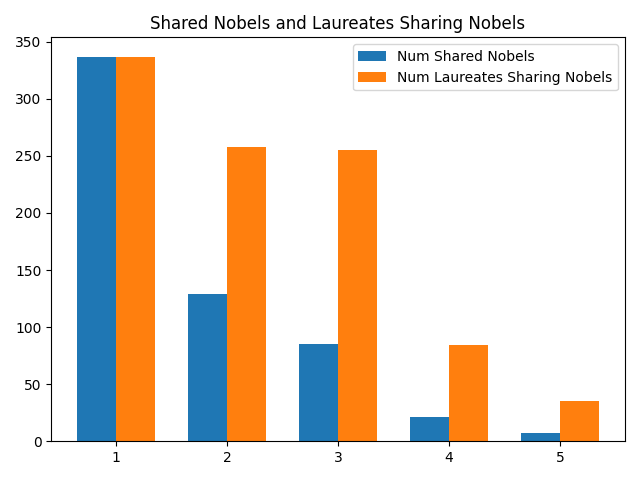
\includegraphics[width=0.7\linewidth]{../queries/plots/prizeShare.png}
	\caption{Graph showing the distribution of Nobel Prizes and laureates.}
	\label{fig:prizeShare}
\end{figure}

\section{Collaborations among Nobel Laureates}

\begin{lstlisting}
PREFIX : <http://www.semanticweb.org/a3d/ontologies/2024/10/nobelOntology/>
PREFIX rdf: <http://www.w3.org/1999/02/22-rdf-syntax-ns#>
PREFIX foaf: <http://xmlns.com/foaf/0.1/>

SELECT ?title (GROUP_CONCAT(?name; SEPARATOR = ", ") AS ?laureates) WHERE {
    ?laureate rdf:type :Laureate .
    ?paper rdf:type :Paper ;
        :hasTitle ?title .
    ?laureate :hasWritten ?paper .
        foaf:name ?name .
}
GROUP BY ?title
HAVING (COUNT(DISTINCT ?laureate) > 1)
\end{lstlisting}

\vspace{1em}

The goal of this query was to explore whether Nobel laureates collaborate with each other by co-authoring
scientific papers. As the table \ref{tab:laureates_collaboration} shows, among approximately 53,000 papers
and 904 laureates, only one paper was found to have been co-authored by multiple laureates.

\begin{table}[H]
	\caption{Paper co-authored by multiple Nobel Laureates}
	\centering
	\begin{tabular}{|l|l|}
		\hline
		\textbf{Title}                                                      & \textbf{Laureates}                   \\ \hline
		\textit{Recursive Robust Estimation and Control Without Commitment} & Lars Peter Hansen, Thomas J. Sargent \\ \hline
	\end{tabular}
	\label{tab:laureates_collaboration}
\end{table}

This result suggests that collaboration between Nobel laureates is extremely rare. However, it is important to
note that this outcome should not be taken as definitive, as the datasets used represent only a portion of all
existing papers and laureates. Nevertheless, it provides an interesting insight into the rarity of such
collaborations, offering a percentage-based perspective on how seldom laureates join forces to produce scientific
work.

\section{How fundings in R\&D affect the possibility for a country to win a Nobel?}

\begin{lstlisting}
PREFIX : <http://www.semanticweb.org/a3d/ontologies/2024/10/nobelOntology/>
PREFIX rdf: <http://www.w3.org/1999/02/22-rdf-syntax-ns#>

SELECT ?year ?topCountry (COUNT(DISTINCT ?laureate) AS ?numLaureates) (SUM(?fundingAmount) AS ?totalFunding) WHERE {
    ?laureate rdf:type :Laureate ;
  	:hasWon ?nobelPrize ;
        :bornIn ?city .
    ?nobelPrize :hasYear ?year .
    ?city :locatedIn ?topCountry .

    OPTIONAL {
        ?topCountry :hasFunded ?funding .
        ?funding :hasYear ?year ;
            :hasAmount ?fundingAmount .
    }
    { # Select country with most laureates
        SELECT (?country AS ?topCountry) WHERE {
        ?laureate rdf:type :Laureate ;
            :bornIn ?city .
        ?city :locatedIn ?country .
        }
        GROUP BY ?country
        ORDER BY DESC(COUNT(DISTINCT ?laureate))
        LIMIT 3
    }
}
GROUP BY ?year ?topCountry
HAVING (SUM(?fundingAmount) > 0)
ORDER BY ?year ?topCountry
\end{lstlisting}

\vspace{1em}

With this query, we identified the top three countries with the highest number of Nobel laureates born there, along with the annual amount of funding allocated to research and development (R\&D) by these nations. To ensure data consistency, we focused exclusively on the years from 2000 to 2016.

\begin{figure}[h!]
	\centering
	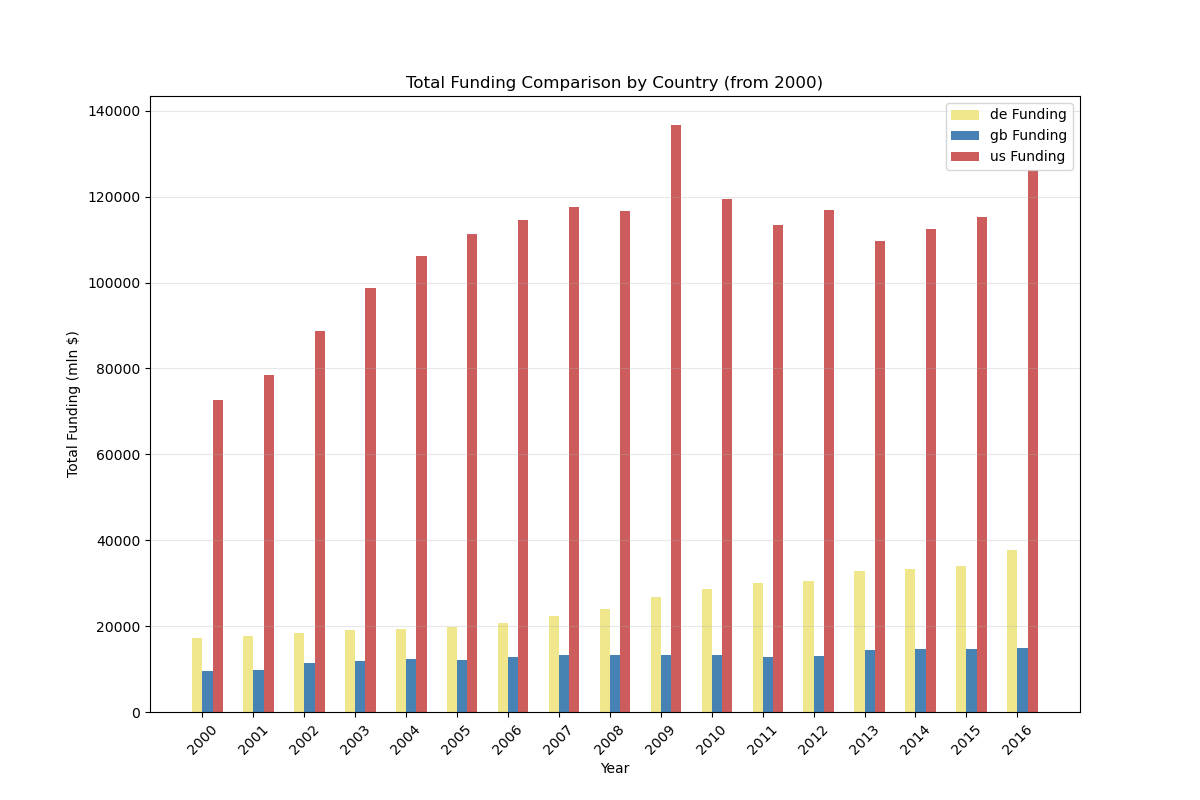
\includegraphics[width=0.9\textwidth]{../queries/plots/funding_comparison_by_country.png}
	\caption{Funding Comparison by Country}
\end{figure}

\begin{figure}[h!]
	\centering
	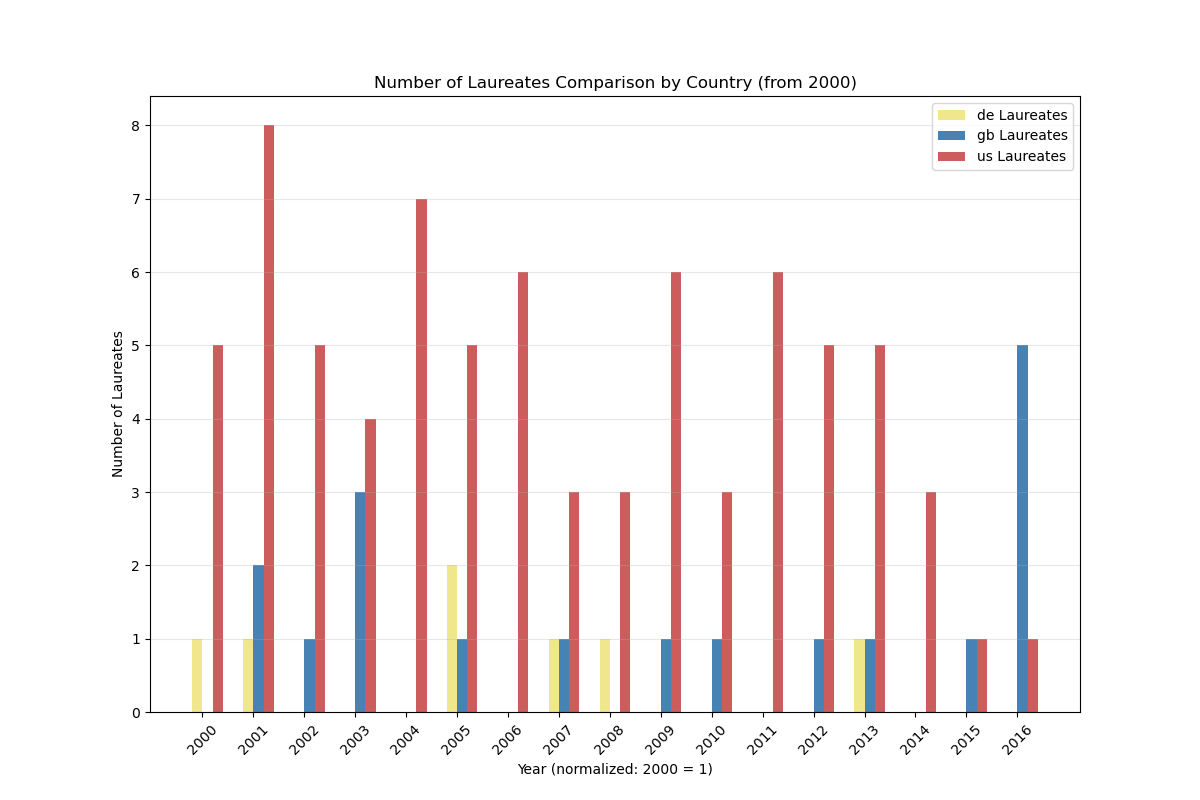
\includegraphics[width=0.9\textwidth]{../queries/plots/laureates_comparison_by_country.png}
	\caption{Laureates Comparison by Country}
\end{figure}

The graphs reveal a strong correlation between R\&D funding and the number of Nobel laureates. In particular, the United States dominates both metrics, demonstrating how substantial investments in research directly contribute to significant achievements in this field, resulting in a higher number of laureates annually.

The situation in Great Britain, highlighted in the following plot, is particularly curious and further supports this observation:

\begin{figure}[h!]
	\centering
	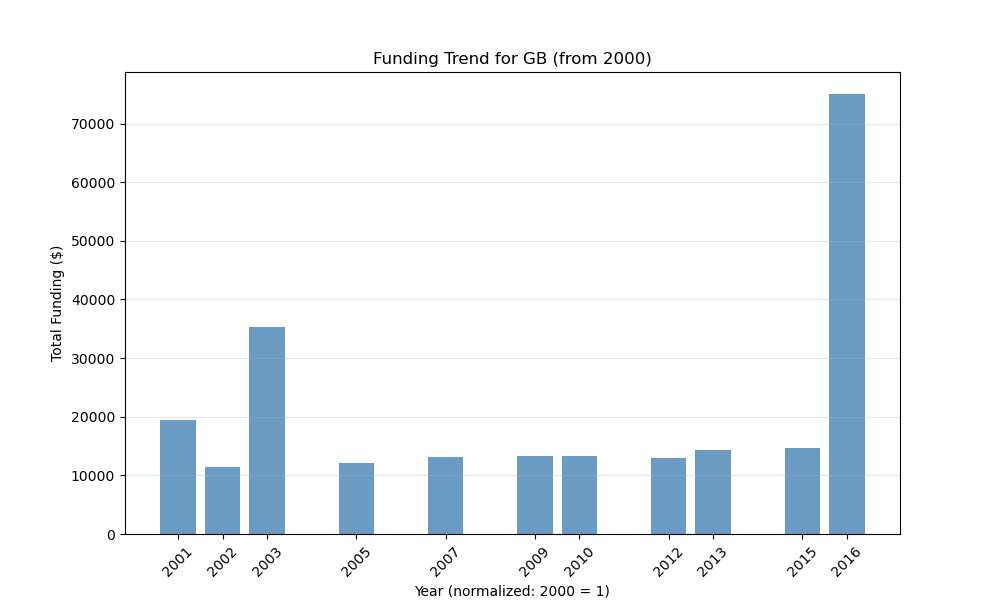
\includegraphics[width=0.9\textwidth]{../queries/plots/gb_funding_trend_bar.png}
	\caption{Great Britain R\&D Funding Trend}
\end{figure}

It's clear that the trends in funding and the number of laureates mirror each other closely. From 2001 to 2003, we observe the same pattern in both metrics. Subsequently, a steady and low level of R\&D funding still reflects the number of British Nobel laureates until 2016, when a sharp increase in Nobel prizes matches with a significant rise in R\&D investments.

\section{moreThanOneNobel}

\begin{lstlisting}
PREFIX spif: <http://spinrdf.org/spif#>
PREFIX rdfs: <http://www.w3.org/2000/01/rdf-schema#>
PREFIX jur: <http://sweet.jpl.nasa.gov/2.3/humanJurisdiction.owl#>
PREFIX skos: <http://www.w3.org/2004/02/skos/core#>
PREFIX foaf: <http://xmlns.com/foaf/0.1/>
PREFIX : <http://www.semanticweb.org/a3d/ontologies/2024/10/nobelOntology/>
PREFIX xsd: <http://www.w3.org/2001/XMLSchema#>

SELECT ?laureate ?numNobels (GROUP_CONCAT(DISTINCT ?category; SEPARATOR = ", ") AS ?categories) WHERE {
    {
        SELECT ?laureate (COUNT(?nobel) AS ?numNobels) WHERE {
            ?laureate :hasWon ?nobel.
        }
        GROUP BY ?laureate
        HAVING (?numNobels > 1)
    }
    ?laureate2 :hasWon ?nobel2.
    ?nobel2 :hasNobelCategory ?category.
    FILTER (?laureate2 = ?laureate)
}
GROUP BY ?laureate ?numNobels
\end{lstlisting}
The query aims to identify Laureates who have won more than one Nobel Prize. By grouping the laureates and counting the number of Nobel Prizes each has won, the query filters the results to show only those with more than one prize.
Table \ref{tab:moreThanOneNobel} shows the output of this query.

\begin{table}[H]
	\caption{Laureates who won more than one Nobel Prize}
	\centering
	\begin{tabular}{|l|l|l|}
		\hline
		\textbf{Laureate}                      & \textbf{Number of Nobels won} & \textbf{Categories} \\ \hline
		Comite International De La Croix-Rouge & 3                             & Peace               \\ \hline
		Frederick Sanger                       & 2                             & Chemistry           \\ \hline
		John Bardeen                           & 2                             & Physics             \\ \hline
		Linus Carl Pauling                     & 2                             & Chemistry, Peace    \\ \hline
		Marie Curie                            & 2                             & Physics, Chemistry  \\ \hline
		UNHCR                                  & 2                             & Peace               \\ \hline
	\end{tabular}
	\label{tab:moreThanOneNobel}
\end{table}

The results highlight the diverse contributions of laureates in different fields, from physics and chemistry to peace and humanitarian efforts. This demonstrates the breadth of achievements recognized by the Nobel Prizes and the multidisciplinary impact of the laureates. \\
Furthermore, the fact that only six laureates have achieved this result serves as a powerful reminder of the Prize's prestige and reflects the long-term impact and ongoing relevance of a laureate’s work.



\section{Number of papers published from the most important venues over the years}

\begin{lstlisting}
PREFIX : <http://www.semanticweb.org/a3d/ontologies/2024/10/nobelOntology/>

SELECT ?venue ?year (COUNT(?paper) AS ?numPapers) WHERE {

    # Get the most important venues (the ones with at least 800 papers published)
    {
        SELECT ?venue (COUNT(?paper) AS ?totPapers) WHERE {
            ?paper :publishedIn ?venue.
        }
        GROUP BY ?venue
        HAVING (?totPapers > 800)
        ORDER BY DESC (?totPapers)
    }

    # get the number of paper published in the most important venues for each year
    ?paper :publishedIn ?venue;
        :hasYear ?year.
}
GROUP BY ?venue ?year
ORDER BY ASC (?year)
\end{lstlisting}

This query returns the number of papers published over the years by major
venues (those with at least 800 papers published, according to our dataset).

Figure \ref{fig:papersPerVenue} shows the trends of the six major research venues.

\begin{figure}[H]
	\centering
	\label{fig:papersPerVenue}
	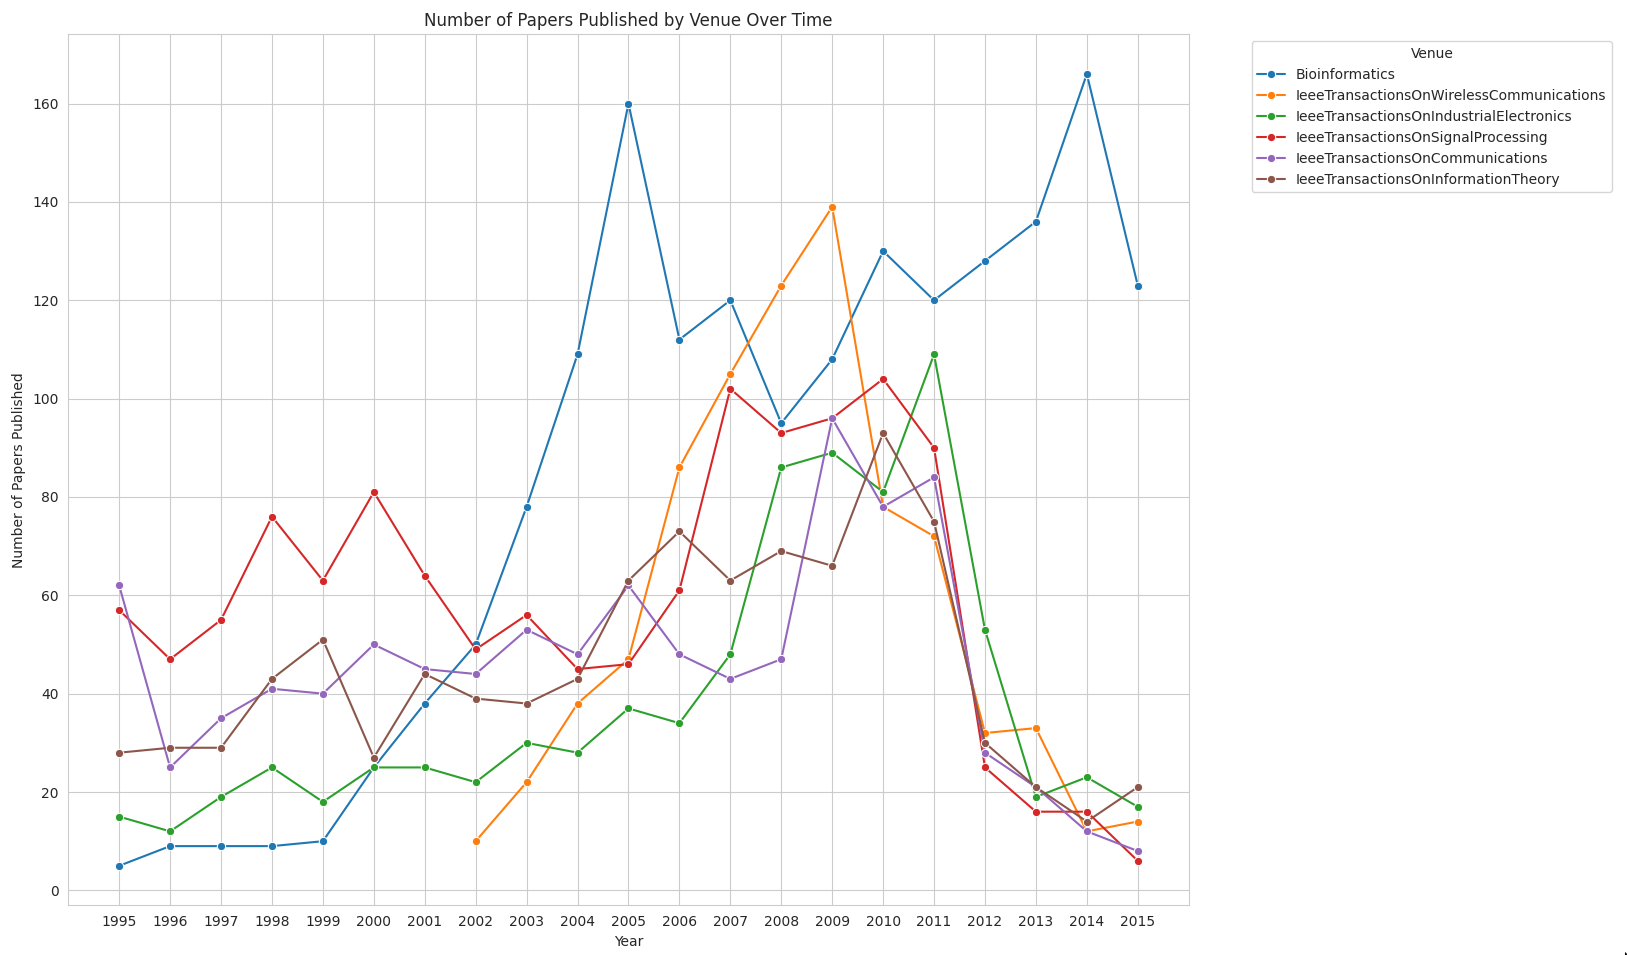
\includegraphics[width=\textwidth]{../queries/plots/papersPerVenue.png}
\end{figure}

In recent years, Bioinformatics could be considered one of the most influential
venue due to its consistently higher number of papers published compared to others.
IEEE venues, are the most prominent in the fields of information and tecnology.\\
For instance, on 2009, the research community focused more on the field of
communications.
That same year, the Physics Nobel Prize was awarded for "groundbreaking achievements
concerning the transmission of light in fibers for optical communication".

\section{papersPerCategory}
The following query allows us to extract, for each year, the number of scientific articles published in each relevant category. The categories returned
as results are the TopConcepts categories of our SKOS taxonomy, and they include in the count their various subcategories. For example, in the count
of papers for the medicine category, articles belonging to subcategories like neuroscience are also included.

\noindent To obtain this data, the query uses two distinct subqueries. The first subquery extracts the number of articles published for each main category
(TopConcept), while the second identifies the number of articles associated with the subcategories of each main category. The sum of the results of
the two subqueries, aggregated by year and category, provides the total number of articles published for each category and for each year.

\begin{lstlisting}
PREFIX skos: <http://www.w3.org/2004/02/skos/core#>
PREFIX : <http://www.semanticweb.org/a3d/ontologies/2024/10/nobelOntology/>
# Extracts the number of papers we have for each category over the years --> the most studied research areas over the years
SELECT ?year ?category (SUM(?howmany) AS ?totalPapers) WHERE {
    # Inner query to extract the number of papers published in journals that have at least one category that is a top concept of our skos scheme
    {
        SELECT ?year ?category (COUNT(DISTINCT ?paper) AS ?howmany) WHERE {
            ?journal :hasJournalCategory ?category .
            :journalCategoryScheme skos:hasTopConcept ?category .
            ?paper :publishedIn ?journal ;
                :hasYear ?year .
        }
        GROUP BY ?year ?category
    }
    UNION
    # Inner query to extract the number of papers published in journals that have at least one category that is a subcategory of a top concept category
    {
        SELECT ?year ?category (COUNT(DISTINCT ?paper) AS ?howmany) WHERE {
            ?journal :hasJournalCategory ?cat .
            ?cat skos:broaderTransitive ?category .
            ?paper :publishedIn ?journal ;
                :hasYear ?year .
        }
        GROUP BY ?year ?category
    }
}
GROUP BY ?year ?category
ORDER BY DESC (?totalPapers)
\end{lstlisting}

\newpage

\noindent This approach offers a comprehensive view of the distribution of published articles over time, allowing us to identify which research areas, related
to Nobel categories, have attracted the most attention from scholars over the years.

\noindent Below is a plot representing the trend of the number of papers published over the years, divided by their respective categories.
In the recent years, the most studied field is medicine which got a big leap around 2002, while in the nineties the most studied one was economics, which
reached its peak in 2008, probability due to the economic crisis of that time.
\begin{figure}[ht]
	\centering
	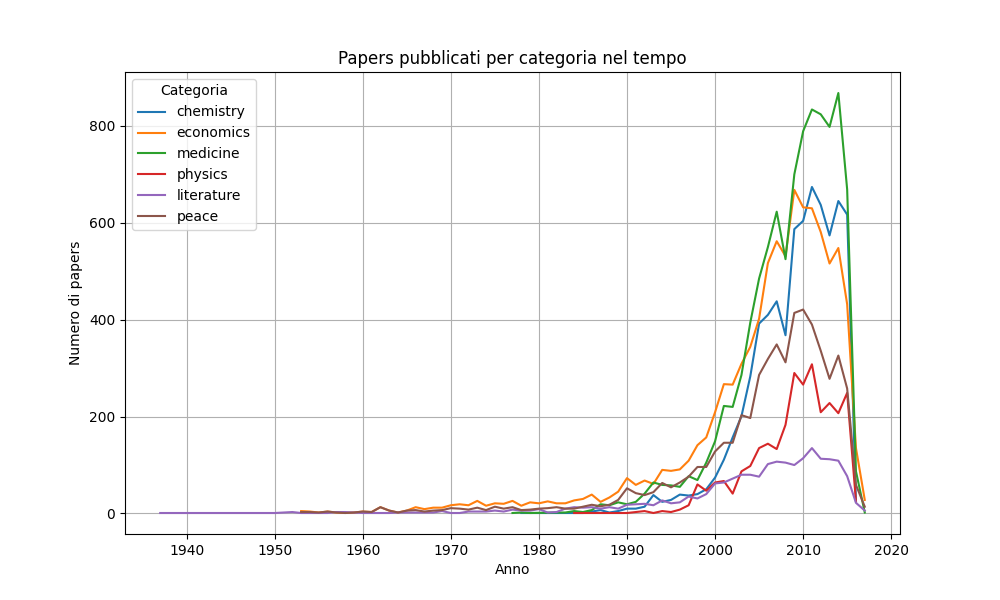
\includegraphics[width=\textwidth]{../queries/plots/papersPerCategory.png}
\end{figure}

\section{Age Analysis of Nobel Prize Winners}
\begin{lstlisting}
PREFIX : <http://www.semanticweb.org/a3d/ontologies/2024/10/nobelOntology/>
PREFIX foaf: <http://xmlns.com/foaf/0.1/>

SELECT ?category (MIN(?age) AS ?maxAge) (ROUND(AVG(?age)) AS ?avgAge) (MAX(?age) AS ?minAge)
WHERE {
  ?laureate a :Laureate ;
            :birthDate ?birthDate ;
            :hasWon ?prize .
  ?prize :hasYear ?prizeYear ;
         :hasNobelCategory ?category .

  BIND (YEAR(?prizeYear) - YEAR(?birthDate) AS ?age)
}
GROUP BY ?category
\end{lstlisting}

The data extracted from the query provides insights into the age at which individuals achieve great results in
their fields:

\begin{table}[h!]
\centering
\caption{Age statistics of Nobel Prize winners by category.}
\begin{tabular}{|l|c|c|c|}
\hline
\textbf{Category} & \textbf{Min Age} & \textbf{Avg Age} & \textbf{Max Age} \\ \hline
Chemistry    & 35 & 58 & 85 \\ \hline
Economics    & 51 & 67 & 90 \\ \hline
Literature   & 42 & 65 & 88 \\ \hline
Medicine     & 32 & 58 & 87 \\ \hline
Peace        & 17 & 61 & 87 \\ \hline
Physics      & 25 & 55 & 88 \\ \hline
\end{tabular}
\label{tab:age_analysis}
\end{table}

\subsection{Observations and Analysis}
The table \ref{tab:age_analysis} highlights notable trends in the ages of Nobel Prize winners:

\begin{itemize}
    \item \textbf{Economics}: With an average age of 67, this category has the highest average age.
    This observation likely reflects the time required to develop groundbreaking theories and gain significant
    recognition in this field. Also the minimum age of 51 suggests that Nobel laureates in Economics often
    achieve their recognition later in life.
    
    \item \textbf{Peace}: This category includes the youngest laureate, at only 17 years old.
    The diversity in ages within the Peace category (average age 61, maximum 87) may reflect the variety of
    contributions recognized, from lifelong efforts in diplomacy to impactful single events, such as activism
    or humanitarian work.
    
    \item \textbf{Chemistry, Medicine, and Physics}: These science-related categories show similar average ages
    (55-58 years) and a range of minimum ages (from 25 to 35 years). The relatively young ages of some laureates
    in Physics (25) and Medicine (32) suggest that groundbreaking discoveries in these fields are sometimes made
    early in a researcher's career, possibly during postdoctoral experiences.
    
    \item \textbf{Literature}: With an average age of 65, second only to Economics, and a minimum age of 42, this
    category highlights the time often required for authors to craft a significant body of work or achieve literary
    mastery. Furthermore, the Nobel Prize in Literature is frequently awarded in recognition of an author's
    entire career, considering their overall contribution to the field rather than a single achievement.
\end{itemize}

By digging deeper into the age data, we performed an additional query to identify the youngest and oldest
Nobel Prize winners. 

\begin{lstlisting}
PREFIX : <http://www.semanticweb.org/a3d/ontologies/2024/10/nobelOntology/>
PREFIX foaf: <http://xmlns.com/foaf/0.1/>

SELECT ?laureate ?name ?birthDate ?prize ?prizeYear ?age
WHERE {
  {
    SELECT ?laureate ?name ?birthDate ?prize ?prizeYear ?age
    WHERE {
      ?laureate a :Laureate ;
                foaf:name ?name ;
                :birthDate ?birthDate ;
                :hasWon ?prize .
      ?prize :hasYear ?prizeYear .

      BIND (YEAR(?prizeYear) - YEAR(?birthDate) AS ?age)
    }
    ORDER BY ?age
    LIMIT 1
  }
  UNION
  {
    SELECT ?laureate ?name ?birthDate ?prize ?prizeYear ?age
    WHERE {
      ?laureate a :Laureate ;
                foaf:name ?name ;
                :birthDate ?birthDate ;
                :hasWon ?prize .
      ?prize :hasYear ?prizeYear .

      BIND (YEAR(?prizeYear) - YEAR(?birthDate) AS ?age)
    }
    ORDER BY DESC(?age)
    LIMIT 1
  }
}
\end{lstlisting}

The results are presented in the following table:

\begin{table}[h!]
\centering
\caption{The youngest and oldest Nobel Prize winners.}
\begin{tabular}{|l|l|l|l|c|}
\hline
\textbf{Name}    & \textbf{Birth Date} & \textbf{Prize}      & \textbf{Year} & \textbf{Age} \\ \hline
Malala Yousafzai & 1997-07-12          & Peace 2014          & 2014          & 17           \\ \hline
Leonid Hurwicz   & 1917-08-21          & Economics 2007      & 2007          & 90           \\ \hline
\end{tabular}
\label{tab:youngest_oldest}
\end{table}

The youngest Nobel Prize winner is Malala Yousafzai, who received the Peace Prize in 2014 at the age of just 17.
Her recognition came as a result of her activism for girls' education and human rights, which gained international
attention and inspired millions worldwide.\\
The oldest Nobel laureate is Leonid Hurwicz, who was awarded the Nobel Prize in Economics in 2007 at the age of 90.
This result demonstrates a lifetime of work in economics, highlighting how breakthroughs in theoretical fields
often come from years and years of efforts and experience.

\end{document}
